95. $\cfrac{(x^2-3x+2)(1-x)}{x-3}\geqslant0\Leftrightarrow\cfrac{(x-2)(x-1)(1-x)}{x-3}\geqslant0\Leftrightarrow\cfrac{(x-2)(x-1)^2}{x-3}\leqslant0.$ Применив метод интервалов, найдём ответ:
\begin{figure}[ht!]
\center{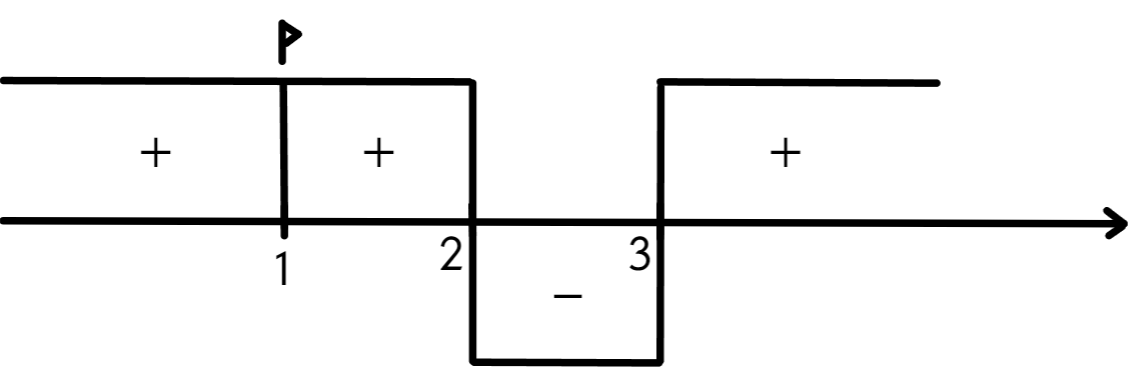
\includegraphics[scale=0.35]{int95.png}}
\end{figure}
$x\in\{1\}\cup[2;3).$\\
